\documentclass{article}

\usepackage{geometry}
\usepackage{makecell}
\usepackage{array}
\usepackage{multicol}
\usepackage{setspace}
\usepackage{changepage}
\usepackage{booktabs}
\usepackage{titlesec}
\usepackage{graphicx}
\usepackage{float}
\newcolumntype{?}{!{\vrule width 1pt}}
\renewcommand\theadalign{tl}
\setstretch{1.10}
\setlength{\parindent}{0pt}
\graphicspath{ {./images/} }

\titleformat{\section}
  {\normalfont\Large\bfseries}{\thesection}{1em}{}[{\titlerule[0.8pt]}]

\geometry{top=12mm, left=1cm, right=2cm}
\title{21W ENM.01512UB American Culture - History and Society VO}
\author{Andreas Hofer}

\begin{document}
	\maketitle
	\section{Intro - 15.10.2021}
	Columbus was obsessed about finding India in the west. He believed that if he went far enough west, he would, on a round planet, eventually end up in India.\\
	Queen Isabella of Castille and Leon and Ferdinand II of Aragon financed Columbus journeys. \\
	It took him two months to cross the Atlantic, where he became Governor of the Indies but was later deported to Spain due to accusations of tyranny. \\
	\subsection{Other Explorers}
	Alvar Nuñez Cabeza de Vaca explored modern Florida and Texas in 1528. \\
	Amerigo Vespucci surmised that Brazil was part of a new continent instead of India, which he named "The New World". \\
	Based on these assumptions German Cartographer Martin Waldseemüller named this new continent after him using his Latinised name "Americus Vespuccius" as, according to him, all explorers before Amerigo did not find a new continent but just more of India. \\
	Amerigos assumptions were proven correct in 1513 when Vasco Nuñez de Balboa reached the Pacific Ocean from Panama. \\
	\subsection{Conquistadores in South America}
	At first explorers and adventurers in service of Spain and Portugal remained in South America exclusively. \\
	\section{North America}
	Modern Day America traces its roots back to the colony of New England. \\
	The first English settlement was called \textbf{Jamestown}, established in 1607. \\
	Early struggles in the settlement included: \\
	\begin{itemize}
		\item{Food Poisoning}
		\item{Food Shortages}
		\item{Recurring battles with the natives}
	\end{itemize}
	Chesapeake Bay near Jamestown was inhabitated by around 14,000 natives. \\
	\subsubsection{Pocahontas}
	\textbf{Pocahontas} (1595 - 1617) was a native american girl, daughter to the chief of the area \textbf{Powhatan} and often described as his favourite daughter. According to the myth, she threw herself in front of her father, who did not want to tolerate teh settlers, becasue she believed there could be a peaceful coexistence. The romance between John Smith and Pocahontas as depicted in the popular Disney movie is generally understood to just be fictional. She showed the settlers which plants were edible and acted as a sort of ambassador between the First Nations and the settlers. In 1614 she married a plantation owner called John Rolfe with whom she had a son. They both stated that their marriage was not out of love but political nature as it was common for her, as daughter of the chief, and European aristocracy to do. Eventually she was captured on a ship, babtised and converted to Christianity. It is unclear if she was forced to do so or not but she assumed the name "Rebecca", after the biblical figure who was "mother of two nations" and visited the British Kingdom for an audience with the queen. Shortly before she was to return to America she caught, what is presumed to be Pneumonia and died. \\
	\subsection{Puritans and Native Americans}
	Puritans are a religious reform movement in the Anglican church. Their aim was to purify it from its Catholic aspects. Puritans are Calvinists and believe in Predestination, the doctrine that all events are an act of divine will. \\
	They were the first people to celebrate Thanksgiving in 1621 to thank god for the good harvest. Nowadays there is the common opinion that this happened in harmony with native americans but it is generally understood that this was not the case. \\
	When European settlers came to North America, there were an estimated 10 to 100 million native americans. \\
	\subsection{Indian Wars}
	
	

	
	\subsubsection{Mexican Immigrants}
	The large amount of Mexican Immigrants in the 1970s are called the "Dreamers" who were brought to the US with their parents when they were young. In 2003 these people were granted a two year residence and working permit, stopping them from being deported to Mexico. \\
	\section{The Civil War}
	The population of the United States in 1790 was, as a reminder, 3.9 million people. But not all of them were citizens with the right to vote or the right to own property. 750.000 or about 19\% of the population were slaves, most of them black people. \\
	In the same year the first Naturalisation Act was passed, which gave "Free White People" citizenship. This meant that only white people who were not slaves or in indentured servitude were entitled to become citizens. This also meant that slaves were excluded from becoming citizens, and thus voting or owning property. In addition free blacks were also not allowed to become citizens. Indentured servants and native americans were also barred from naturalisation. Later Chinese were excluded as well when the Chinese Exclusion Act was passed. \\
	When America was discovered slavery had already been accepted as a part of society with Rome and Ancient Greece already having held slaves. In 1500 81.000 slaves had been traded to Europe, the Atlantic and Muslim merchants. At first slaves were only traded to South America. \\
	This changed in 1619 when 20 slaves arrived in the British Colonies in Virginia. This was enabled through the legalisation of Chattel Slavery, which meant humans could be considered property. In addition in 1662 Virginia passed a law to have children born to slaves also become slaves. \\
	All of the south of the British Economies relied heavily on slave labour. Between the years 1790 and 1860 the cotton production increased exponentially, in accordance with the amount of slaves. \\
	The production of these goods were introduced in a trade triangle. In America the slaves would produce sugar and cotton, which was sold in Europe to buy Rum and Tobacco, which was in turn brought to Africa and used to buy more slaves to be brought to America. These slaves were brought to America throught the so called \textbf{Middle Route}. \\
	During the Revolution from 1775 to 1783 the Former British Colonies banned the African slave trade. This was done because they refused to trade with the British Empire and not because of moral reasons. \\
	In 1808 the slave trade was abolished nationwide. This did not abolish slavery though and over the next decade the domestic slave-trading industry started an organised slave breeding economy to sell children to other slavers. \\
	In 1850 the percentage of slaves of some of the southern states reached as much as 90%.
	\subsection{Compromises}
	In 1820 the \textbf{The Missouri Compromise} was reached, which prohibited slavery north of the 36th parallel, which included states like Kentucky, Virginia or Maryland, except for the state of Missouri. \\
	In order to have an equal number of pro and against slavery states the state of Maine was created from parts of Massachusetts. \\
	In 1854 the \textbf{Kansas-Nebraska Act} was ratified which annulled the Missouri Compromise when Kansas and Nebraska were opened for settlement and pro slavery even though they were north of the 36th parallel. This led to slavery being up to the sovereign states. \\
	In 1854 the \textbf{Bleeding Kansas} war erupted between anti and pro slavery advocates, between the towns of anti-slavery \textbf{Lawrence} and  pro-slavery\textbf{Lecompton}. \\
	In 1856 James Buchanan was elected, who sought a policy of appeasement with the south. \\
	In 1850 the \textbf{Fugitive Slave Act} was enacted federally, where a hunter who caught somebody helping a slave escape was awarded 10\$ and the slave had no right to a trial. \\
	Harriet Beecher Stowe wrote the book titled \textbf{Uncle Tom's Cabin} which is commonly seen as the trigger to the Civil War. \\
	In 1857 the \textbf{Dred Scott Decision} was made and stated that a slave from Missouri living in a Free State could not achieve his freedom, despite living in a free state. Living in a free state meant that a slave had to be returned to the slave state. This was later nullified by the \textbf{Emancipation Act}. \\
	The movement to abolish slave trade was called \textbf{Abolitionism} who sought to set all slaves free. The two most well known representatives of abolitionism were \textbf{William Lloyd Garrison} and \textbf{Frederick Douglass} who founded the \textbf{American Anti-Slavery Society}. Frederick Douglass was also the most photographed American in the 19th century. \\
	\subsection{The Antebellum South}
	The South consisted of rich plantation owners who grounded their wealth in slave labour. The south was mainly a rural area with few industrialised zones, which was also a reason why they lost the war. The north could simply produce many more weapons than their adversaries. The south is still occasionally seen through a romanticised lens with content slaves and well-dressed "belles" strolling through the midsummer shade. "Gone with the Wind", a movie from 1939, is an example of that talking about "Cavaliers and Cotton Fields [..] where Gallantry took its last bow." \\
	Nowadays \textbf{The Black Belt} is where there is a major black population, ranging from Texas to Virginia with some counties having more than 50\% black people. Despite what it may sound like, the Black Belt is not named after black people but after the black soil of that area. \\
	There was also the \textbf{Great Migration}. In 1910 83\% of black people lived in the South, while in 1970 60\% lived in the North. This was because the Jim Crow laws persisted for a long time in the southern states, and legislation that decreed that slaves living in a free state for a certain amount of time were to become free. \\
	Another part of the south is the \textbf{Bible Belt}, a South-Eastern area with a high rate of Evangelical Protestantism. In Alabam, for example, 94\% population considered themselves religious.\\
	This is in contrast with the \textbf{Mormon Corridor} in Utah where followers of the Church of the Latter Day Saints form a loose net of reformist churches. \\
	\subsubsection{African American Activism}
	In 1791 there was a successful uprising in St. Domingue in Haiti as well as an uprising in "Gabriel's Rebellion" in 1800, a plot in Richmond, Virginia which possibly involved 1100 slaves. There was also "Matt Turner's Rebellion" in 1831 a slave revolt in Southhampton, Virginia. \\
	Other forms of activism were Grassroot Moevements: In the 1850s the \textbf{Underground Railroad} was used to escape the south. They were a network of secret routes and sanctuaries which led to free states or Canada. By 1850 an estimated 100.000 slaves had escaped through the Railroad. The most well known person in the Railroad was \textbf{Harriet Tubman} who was a former slave from Maryland. She is currently debated to become the face of the 20\$ bill in 2030. She would become the 2nd ever woman on American paper currency. \\
	\subsubsection{Other events preceding the Civil War}
	In 1859 John Brown organised an insurrection where he and 18 supporters captured a Federal Weapons Arsenal in order to mount an insurrection. When he was captured and sentenced to death he said: "\textit{I am now quite certain that the crimes of this guilty land will never be purged away but with blood"} which portended the Civil War 1.5 years later. \\
	In 1860 Abraham Lincoln became president with 40\% of the votes. This only happened because the south was split between two candidates, getting 29\% and 13\% of the votes. \\
	Lincoln, a former barkeeper, lawyer and Whig party leader was nominated for Senate by the Republican Party where he gave a famous speech talking about how the house cannot forever stand divided between slave trade and free states. \\
	\subsubsection{Prelude to the Civil War}
	In 1861 the southern states declared their independence from the union. They called themselves the \textbf{Confederate States of America} with South Carolina, Mississippi, Florida, Alabama, Gerogia, Louisiana and Texas being their founding members. They chose the Confederate flag, a blue cross with white stars on a red background. They chose Jefferson Davis as the president of the Confederacy. He was a Democrat, which at that time was a pro-slavery party. \\
	\subsection{Outbreak of the Civil War}
	The first point of aggression was the attack on \textbf{Fort Sumter} on the 12th of April 1861, a base on an island in the bay of Charleston, South Carolina. The Confederacy argued that the fort was on Confederate ground. They eventually took the fort and destroyed it, albeit without killing anybody. \\
	Following this, Virginia, Arkansas, North Carolina and Tennesse seceded as well and joined the Confederacy. \\
	The main battlefields of the Civil War were the battle of Antietam on the 17th of September 1862. This became the bloodiest battle in American history with 22,717 people dead on a single day.
	Another battle was the battle of Gettysburg which took place over the duration of three days. \\
	The Civil War is, to this day the bloodiest battle fought by the USA with 625,000 people having died in it. This meant that 2\% of the population were killed within 4 years. On average 625 people died every single day.\\
	\subsubsection{War "Heroes"}
	One person lauded during the Civil War was \textbf{Ulysses S. Grant} insisting on the unconditional surrender of the South. He became to be known as the "Butcher" after mounting casualties in Virginia. He became President after the Civil War concluded.
	His adversary was \textbf{Robet E. Lee} who was Senior Military Adviser in the Confederacy. He later signed the unconditional surrender Ulysses S. Grant vied for. Despite that he is still remembered with great admiration within the south with statues being erected and streets being named after him. \\
	\subsubsection{Photography}
	With the civil war photographers started being used regularly and the people of the north started seeing the result of battles within newspapers. These were used to give written reports credibility. \\ \\
	In 1865 the 13th Amendment was ratified and slavery was officially ended. \\
	\section{Going West - 19.11.2021}
	It took approximately 6 months to make the journey from the Appalachian Mountains to California. \\
	One of the most famous cases of settlers going west was the \textbf{Donner Party} where from the 87 people trying to go west, only 45 survived after they were caught in a terrible winter in the Sierra Nevada. They survived by resorting to cannibalism. \\
	In total approximately 20,000 settlers died while trying to make their way westward. \\
	\subsection{The Frontier}
	The frontier describes the ever shifting border towards the west, where settlers would claim new land, taking land from the wilderness. The Frontier and its \textbf{Frontier Thesis} was devised by Frederick Jackson Turner, who connected it to American character of an ever-shifting frontier. He described the existence of free land and an advance of settlers as an integral part of American character. \\
	\subsubsection{Wild West Shows}
	Eventually they did run out of land though. And with it came the romanticisation of the Wild West and with that the inception of staged events called \textbf{Wild West Shows}. William "Buffalo Bill" Cody wanted to exploit this infatuation of the population with the wild west. He toured with shows through America and even Europe, where white people but also American Natives showed prop battles and lasso shows to entertain the masses. While not historically accurate, as the wild west was often connected to massacres. Another famous person \textbf{Annie Oakley} a female sharpshooter, which was a rarity, was enlisted by said Buffalo Bill, to star in these shows. Over the years over 100 million people watched these Wild West Shows. Even the Queen of England attended one of them to see what it was about. \\
	\subsection{First Major Expeditions}
	The first major expedition to the west was the Lewis and Clark Epxedition. It was, at first, secret financed by President Thomas Jefferson. The expedition was officially named the \textbf{Corps of Discovery} and started in May 1804. During their journey they were aided by a 16 year old Shoshone woman, who acted as a guide and translator. This expedition increased the knowledge of the Louisiana Territory and the Oregon Territory. \\
	Another famous explorer was \textbf{Zebulon Pike} who mapped the upper Mississippi Area. \\
	\subsection{Independent Republic in the USA}
	Between 1836 and 1846 Texas was an independent state. Still today, many inhabitants consider themselves independent from the United States. In 1835 the Texas Revolution took place, which established itself as a Renegade Republic. In 1845 they were annexed by the US Government and incorporated into the union. This spirit of independence is still visible today, considering that the state is still called the \textbf{Lone Star State}. \textbf{Sam Houston} the hero of the Texas Revolution is one of the most cherished people in Texas, who was the President of the Republic of Texas and later Senator to Texas. \\
	\subsection{Manifest Destiny}
	Puritan settlers had stated that they were portended to take these lands and this was continued until 1845, when \textbf{Manifest Destiny} was established in order to justify the annexation of Texas. By saying that god wants them to do things they could claim all their Imperialist notions to be just. The painting \textbf{American Progress} by John Gast, depicts the zeitgeist of this time, with the manifestation of the continent, Columbia, bringing light to the new lands, bible and telegraph line in hand. \\
	\subsection{Albert Bierstadt}
	He was one of the most prominent painters of that era. A representative of the \textbf{Hudson River School}, painted massive pictues following the \textbf{Luminism} style. In his paintings, it is always a landscape with light coming from the heavens, shining on the far away area, as if God was giving his ok, to taking this land. In 1864 during the New York Fair, his picture "On the Rocky Mountains" was accompanied by 19 mutely standing Native Americans. While this could have been interpreted as a protest, this was part of the exhibition to make it more "realistic". \\
	The Hudson River School was an art movement romanticising the country to celebrate the land and its newly found patriotism. \\
	\subsection{Westward trails}
	Between 1821 and 1880 the Santa Fe Trail was an important route to transporting goods westward. It was a commercial and military transportation route connecting Santa Fe, which is in modern-day New Mexico, to Independence in Missouri and the Missori river, where wares were loaded from and to ships.\\
	Another trail from the Missouri River and the most important trail towards the west was the \textbf{Oregon Trail}, which was 2000 miles in length, connecting the Missouri River and the valleys of Oregon. It was part of the \textbf{Great Migration} where in 1843 approximately 1000 settlers used the trail to settle the Oregon Valley. \\
	Another very important road towards the west was \textbf{Route 66} established in the 1930s leading from Chicago in Illinois (Great Lakes) to Santa Monica in California. It is also called \textbf{The Mother Road} and considered "The main Street of America". During the \textbf{Dust Bowl}, a period of severe droughts, it was used by many settlers to get to California. The droughts were caused by violent storms from the east, after a lot of vegetation was cut down in order to make it ready for settlement. In the state of Oklahoma alone, 15\% of its population left for the west, which increased the popularity of the Route 66. This disaster was one of the main reasons why the US government started having a greater influence in soil and vegetation conservation leading to the foundation of the \\
	\subsection{Gold Rush}
	On the 24th of January 1848, gold was found near a mill in Sacramento which caused the Gold Rush. Over the next years 300,000 people came to California to find more gold. In 1849 alone 90,000 people arrived there. These are called the "Fourty-Niners", not to be confused with the "Fourty Eighters", the German immigrants. \\
	\subsection{More Independence}
	In 1846 California declared indepence in the \textbf{Bear Flag Revolt} mainly by rebellious white settlers. Today with 38 million inhabitants, California is the most populous state of the US. \\
	\subsection{Mexican-American War}
	After Texas was annexed in 1845, the Mexico-American War erupted, as Mexico considered Texas its property. US-American troops invaded New Mexico and California, and even went as far as taking Mexico City. \\
	\subsection{Purchase of Alaska}
	In 1867 the US purchased Alaska, which is 1,7 million km\textsuperscript{2} in size for only 7.2 million US Dollars, which equated to 2 cents per km\textsuperscript{2}. While it is the largest state by land, mass it is also the second least populous state. The least populous state is Wyoming. They have winter in June, apparently. \\
	\subsection{Horse Rapid Mail Delivery}
	In 1860 the \textbf{Pony Express} was established as rapid mail delivery service. While it only lasted for 9 months, it is still remembered today. It transported messages between Missouri and California. It consisted of 150 station about 15 miles or 24 km apart from each other. Candidates for the Pony Express were required to not weigh more thsn 57 kg in order to not tire out the horse too much. In 1861, the Pony Express was replaced by the Transcontinental Telegraph, which made it obsolote. \\
	\subsection{Homestead Act}
	In 1862 Abraham Lincoln signed the Homestead Act to give applicants the right to claim a yet unclaimed area of 160 acres (Later increased to 640 (2,4km\textsuperscript{2})) and have it become their property if they used it for a period of six years. This time period could be reduced to 6 months if you paid a fee of 1.25 Dollars per acre (So a total of 200 Dollars). Until the law was repealed 10\% of the total US Area was distributed through this act. \\
	\subsection{Winchester rifle}
	The Winchester rifle was one of the earliest repeating rifles, allowing the shooter to shoot several times, without having to reload. It was bought from Smith and Wesson by Oliver Winchester, as the "Volcanic Rifle", and perfected it. It remained the most popular gun in America throughout World War I. \\
	\subsection{Promontory Point}
	In 1869 the \textbf{Transcontintental Railroad} was completed and ended at Promontory Point. A man called \textbf{Theodore Dehone "Crazy" Judah} envisioned crossing the Sierra Nevada massive. 90\% of the workforce that built the Transcontinental Railraod were Irish and Chinese men, handling dnagerous substances on a daily basis. \\
	\subsubsection{Fort Astoria}
	On 1811 the first trading post on the Pacific was founded.
	\subsection{Wyatt Earp}
	\textbf{Wyatt Earp} is an iconic figure in folk history. He lived until the old age of 89 despite having been a farmer, a cow puncher, gambler, miner, buffalo, hunter and boxing referee.\\
	\subsection{The Battle of little Bighorn}
	This battle was one of the major victories against the settlers, and is also called General Custers last stand.
	The last fight against natives took place at the \textbf{Battle of Wounded Knee}. A massacre aimed against a number of tribes and was the last push against the settlers. After this the frontier was closed. \\
	\subsection{Voting rights for Women}
	In 1869 Wyoming gave voting rights to women in order to attract women to the state. It was also the state with the first female governor. \textbf{Liz Cheney} is the best known governor from Wyoming, despite being Conservative, she voted for Trumps impeachment and was expelled from the party because of it.

	\section{7th Session - Urbanity and Civilization - 26.11.2021}
	The time span is from the "City upon a Hill" to the Postmetropolis today. Whenever we imagine american cities we imagine large shopping streets, bustling streets and large skyscrapers but this has not always been this way. \\
	It started with Puritanism in the 17th and early 18th century. Very early, when it was still a British colony, they regarded themselves as a beacon of the world. They considered themselves more liberal, more moderated and just in general more virtuous. Despite these views they were still fully dependent on the British Empire. \\
	But this view of being "fully free", like freedom of speech and religion, were marred by a series of epidemics like Smallpox, Yellow Fever and Influenza. This made larger cities less popular as compared to small settlements. Thomas Jefferson stated, that he believes that Yellow Fever especially discourages the formation of larger cities. \\
	\subsection{Suburban areas today}
	While there are 329 million people living in the USA today, 84\% of its population live in urban or suburban areas. This was a marked increase from 69\% in the 1960s. Globally, on average, only 55\% of people live in urban areas so the US can be considered an urban nation. \\
	If we look at the most populous cities in the US, there can be a stark difference between a city's popularity and its population. Miami, for example, which gets a lot of attention only has 442,000 inhabitants which makes it the 44th largest city. Similar to Atlanta, Georgia and Las Vegas in Nevada with 499,000 and 642,000 inhabitants respectively. Detroit, Michigan, with 639,000 inhabitants is the only city in the country with a double-digit shrinking population. This is due to the receding influence of the car industry. \\
	The 10 most pouluous cities in the US are:
	\begin{itemize}
		\item[10.]{San Jose, California}
		\item[9.]{Dallas, Texas}
		\item[8.]{San Diego, California}
		\item[7.]{San Antonio, Texas}
		\item[6.]{Philadelphia, Pennsylvania}
		\item[5.]{Phoenix, Texas}
		\item[4.]{Houston, Texas}
		\item[3.]{Chicago, Illinois}
		\item[2.]{Los Angeles, California}
		\item[1.]{New York, New York - "The City that never sleeps"}
	\end{itemize}
	While these are the largest cities by population, Anchorage in Alaska, with 291,000 inhabitants has a land mass of 4,415 km\textsuperscript{2} which makes it the largest city in terms of land mass. By comparison, New York only has a land mass of 700 km\textsuperscript{2}. \\
	If you look at a popluation map of the US, you can see that population mostly concentrates on the coasts, with a few notable exceptions like Chicago. \\
	\subsection{New York - New Amsterdam - Gotham}
	When New York was founded it was not called that but \textbf{New Amsterdam} as at that time the area was considered the \textbf{New Netherlands}. It was founded in 1626 by the Dutch as a fur trading outpost but later became a British Colony and was renamed to New York.
	In the Lenape language, which was the tribe that lived in Delaware, \textbf{Mannahatta} was called "The Island of Many Hills". It was part of the \textbf{Lenni Lenape Territory} in the early territory. \\
	According to legend, as it has been put into doubt by historians, in the year of 1626 the Dutch bought Mannahatta from the Lenni Lenape for 60 Guilders, which was 24\$ and is equivalent to 1,000\$ today. \\
	In 1789 New York became the first US-American capital. There are three capitals in the history of the United States and New York city was its first capital. When the Constitution came into effect in 1789 New York became its official capital. It was New York's federal hall, where the first seat of Congress was placed. In 1790 the capital was changed to Philadelphia and was changed again in 1800 to Washington D.C. \\
	In 1825 the \textbf{Erie Canal} was opened, a 363 mile long canal connecting the Hudson River to the Great Lakes in the north and made it possible for the cities in the west to trade with New York. \\
	In 1885 New York was the first American city to release a daily newspaper in Yiddish called "Tageblatt". It was an orthodox, religious newspaper. There has, historically, been a large amount of Jewish people living in New York. There are an estimate of 980,000 Jewish people living in New York today, which is about 12\% of hte population. This is even higher in Manhattan, where 20\% of the population are of Jewish origin. This does not mean that they actively practice the faith but just have a Jewish background. This makes New York the largest Jewish settlement in the world, only after Tel Aviv. \\
	The New York Subway System, which is the largest in the world, has 472 stations with 14 still planned. There's 842 miles of tracks(1,355km).
	Before the subway became popular, \textbf{Horsecars}, which are railroads pulled by horses, were the most popular vehicles of mass transit until the cable car came along. San Francisco had the first cable car, which is just a car pulled by a cable. \\
	In 1857 toilet paper was invented by Joseph C. Gayetty calling it "Perforated Paper". This was a major breakthrough as sanitary standards were abyssmal. Many New Yorkers lived in so called \textbf{Tenements} which were dark, crowded buildings with multi-family apartments. \\
	\begin{figure}[H]
	\centering
	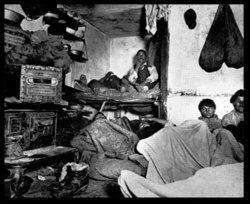
\includegraphics{Tenements.png}
	\end{figure}
	
	The Ashcan School was a painting school showing the poverty in urban areas.
	Opened in 1895 the \textbf{Lombardi's} claims to have been the first Pizzeria in America. This claim is disputed. \\
	New York city today is the safest city of the largest 7 cities. The crime rate in New York has continually increased, at one point having been the safest of the largest 25 cities.
	By comparison, the city with the highest homicide rate is St.Louis in Missorui with 66.07 per 100,000 people. Missouri is also called the "Show-Me" state.
	\subsection{Chicago - The Windy City}
	Chicago is called the Windy City, even using that in advertisement. \\
	In 1885 Chicago had the first Skyscraper, the Home Insurance Building, which cannot really be called a modern skyscraper, with only 42m in elevation.
	\subsection{New Orleans - The Big Easy}
	New Orleans is called \textbf{The Big Easy}, built on the Mississippi River Delta, with half of the city being beneath sea level. Until 1800 it was property of Spain but then ceded to France. Only 3 years later in 1803 it became part of the USA with Louisiana Purchase. It is known for its Mardi Gras festival. \\
	\subsection{San Francisco - Yerba Buena - Phoenix from the Ashes}
	San Francisco was established by Spanish Missionaries in 1776 then called Presidio (Which is still a district of the city). The herb Yerba Buena was used as a namesake of the settlement. It became part of the USA in 1846 after the Mexican-American War and renamed to San Francisco. In the Gold Rush 1848 it became a magnet for the 49ers immigrants. In 1850 of the 25,000 people there were only 300 women in the city. It is called "Phoenix from the Ashes" because the city has burned down 4 times. Until today one of the fires which cost 3,000 people their lives is the most lethal disaster in the history of California. \\
	\subsection{Los Angeles - Hollywood}
	Los Angeles, which only had 5,000 inhabitants in 1870, is the 2nd largest city today, which it has been since the 1980s. Hollywood, which used to be a small independent agricultural community, decided to merge with Los Angeles in order to gain access to the sewer system. Before it was annexed by the US movie theaters were banned there. After 1911 Hollywood became the centre of the U.S. motion picture industry. The sign which has been erected in 1923 originally used to read \textbf{Hollywood Land} but was later changed to just Hollywood after there were numerous suicides from the D of the sign, since it had 13 letters, which was considered bad luck. \\
	\subsection{Vertical Building}
	Over time, vertical building became much more popular. One invention to make this possible was the elevator, invented by Elisha Otis in 1852. Between 1931 and 1972 the Empire State Building was the largest building in the world.
	Another big factor was the production of steel. While originally very hard to produce, \textbf{Andrew Carnegie} founded Carnegie Steel Company and allowed for the cheap and efficient production of steel. This allowed for new things, like skyscrapers. \\
	
	\section{Imperialism and Ideology - 03.12.2021}

	Imperialism started in 1820, when the \textbf{Monroe Doctrine} was enacted. The Doctrine is a policy of mutual non-interfence between the USA and Erope. Because of that the USA considered any effort made by a European nation to colonize land in North or South America an act of aggression. Their aim was to keep all European nations from gaining control in any part of the Americas. It is named after \textbf{James Monroe}(1758 - 1831) who was a founding father and the 5th President. He was the third former president, after John Adams and Thomas Jefferson, to die on the 4th of July, the US national holiday. \\
	While the US did not want any outside interference to the Americas, the \textbf{Westward Movement} continued unabated, cuasing great losses to Native American population. It had an estimated population of at least 10 million but at most 100 million separated in over 500 tribes, each with their own culture, when the settlers arrived. \\
	While the US policy towards Native Americans was marked by diplomacy, they were often just gotten rid of. In the \textbf{Indian Removal Act} enacted by Thomas Jefferson, Native American tribes were removed from their homeland and moved to reservations where they could be controlled by the government. \\
	In 1823 the \textbf{Cherokee Nation} was formed by the members of the Cherokee tribe. They had their own constitution and currency. Nevertheless were they removed from their original homeland to plateaus in Missouri and Oklahoma. The Cherokee were part of the \textbf{"Civilised Tribes"}, the Cherokee, the CHikasaw, Choctaw, Creek and Seminole. According to a census in 2000 the Cherokee is the largest tribe of Native Americans with 563 recognised members. \\
	This series of forced relocations happening in 1831 is called the \textbf{Trail of Tears}. The tribes most affected were members of the Cherokee, the Muscogee, the Seminole, the Chickasaw and Choctaw. During this relocation 60,000 Native Americans died. This also includes the 2000 African American Slaves the Native Tribes held. \\
	\subsection{New US-Imperialism}
	In the 1890s US diplomacy started reaching beyond the mainland of North America. This can be sectioned into three steps:
	\subsubsection{Hawaii}
	In 1893 Queen Lili'uokalani was overthrown by a "Committee of Safety" consisting of American and European citizens. Hawaii was considered an important economic position in the pacific, since it was one of the only stops in the Pacific for merchant vessels.
	President William McKinley, who was strongly imperialist, signed the \textbf{Newlands Resolution} which led to the annexation of Hawaii in 1898.
	\subsubsection{Cuba}
	Cuba was for the longest time a Spanish Colony with a significant production of sugarcane. In 1868 Cuban nationalists declared independence which led to a ten-years war against Spain. Until 1896 General Weyler, also called the Butcher, violently put down resistances. In 1898 the US government sent the Maine to Cuba to "rescue Americans" which exploded in Havana and killed 266 people. \\
	This led to the \textbf{Spanish-American War} from 1898. It is also often referred to, mainly by American Jingoists, the "Splendid Little War". \\
	The war ends at the end of 1898 with the Treaty of Paris, after which Cuba becomes independent. In turn Puerto Rico is annexed and becomes a prtoectorate of the USA. This meant that Puerto Ricans had no contitutional rights and were not granted citizenship until 1917. \\
	\textbf{Theodore "Teddy" Roosevelt}, an influental president of the US. He graduated from Harvard University in 1880 and joined the Rough Riders when the Spanish American War started. He is lauded a war hero from the Battle of San Juan Hill in July 1898. When he returned he became Governour of New York from 1899 to 1900 and US Vice-President in 1901. When William McKinley was assassinated shortly after he became President. He was the youngest president ever at Age 42. (John F. Kennedy was 43 when he was elected). \\
	Another thing named after Roosevelt is the Teddy Bear, a soft toy, first presented in 1903. In the myth Roosevelt spares a bear from being shot, which was later marketed in the media and caused somebody to make the Teddy Bear in his honour. \\
	\subsubsection{The Philippenes}
	In 1896 there is an insurrection against the Spanish colonizers. The rebel leader \textbf{Emilio Aguinaldo} considered the US their allies and asked them for help. Due to that the US end up buying the Philippines in 1898 for 20 million \$ . This resulted in the \textbf{American-Phillipine War} where Aguinaldo, now in power, fought agains American troops. \\
	\subsection{Other Events around 1900 concerning US Imperialism}
	The \textbf{Boxer Rebellion} in 1900 was a nationalist and anti foreign rebellion in China which killed 200 foreigners. As a reaction the \textbf{Eight-Nation Alliance} was formed and takes control of China with 20000 amred troops. This had the US gain access to the lucrative market of China. \\
	\subsubsection{Panama Canal}
	In 1903 a US treaty with Panama had the Panama Canal built, an 80km long canal through Middle America. It cost 390 million \$ and used 40000 workers. \\
	\subsection{World War 1}
	The US only got involved very late into WW1 from 1917 to 1918. Despite this short time it was one of the bloodiest wars the US ever fought where of the 4 million soldiers serving as military personnel, 110.000 were killed. President Woodrow Wilson, who reigned from 1913 to 1921, famously said "War Should bring Democracy and reform to the whole world" which tries to justify the Imperailist attitudes by the US. \\
	\subsection{The Roaring Twenties}
	The Roaring twenties were an economic boom happening between 1920 and 1929. This era ended with the \textbf{Black Tuesday} where a stock market crash happened due to an asset bubble of the 1920s, where the Dow Jones Index fell by 25%. \\
	\subsection{The Great Depression}
	After the 1920s the Great Depression followed, where unemployment and poverty
	\subsection{The Thirties - The Red Decade}
	The 1930s were also called the \textbf{The Red Decade} for the predominance of socialist ideas in the USA. Franklin D. Roosevelt enacted the \textbf{New Deal}, which was in opposition to the previous laissez-faire attitude of the government concerning business practices, as he did not expect the Great Depression to rectify itself. The program restored the US economy as a response to the Great Depression using "socialist ideas". \\
	This was marked by the "Three Rs":
	\begin{itemize}
		\item{Relief}
		\item{Recovery}
		\item{Reform}
	\end{itemize}
	\subsection{World War 2}
	In 1939 World War 2 erupted with the invasion of Poland. This led to two major alliances:
	\begin{itemize}
		\item{The Allies: Poland, France, Great Britain, the US and the USSR}
		\item{The Axis: Germany Italy and Japan}
	\end{itemize}
	The US only entered World War 2 in December 1941 as a reaction to the Attack on Pearl Harbor, a navy base in Hawaii, by Japanese forces. Within the US this led to totalitarian measures, where Japanese descendands living in America were put under general suspicion and put into internment camps. \\
	In May 8th 1945 "VE-Day" is celebrated, when Berlin is taken by Allied forces. Later in August 14th "VJ-Day" happened, when Japan surrendered. \\
	\subsection{Cold War}
	After World War 2 the \textbf{Cold War} soon came to pass. While there was no armed conflict, it was a tense conflict between the two Superpowers: The USA and the USSR. Despite there being no direct wars between the two powers there were proxy wars, with both sides supporting enemies in an armed conflict. The cold war was also marked by the \textbf{Iron Curtain}, a border between the Western and the Eastern sphere. This border was guarded by walls and guards, which kept people from leaving or entering. \\
	\subsubsection{Nikita Khrushchev}
	Nikita Khrushchev was the Soviet Leader between 1953 and 1964. He is known for his words of "We will bury you", which threatened a real armed conflict. \\
	In 1991 the Cold War ends with the USSR dissolving into many parts. This was preceded by measures such as \textbf{Perestroika and Glasnost} in 1985 as well as the Fall of the Berlin Wall and the Iron Curtain in 1989, when Ronald Reagan said: "Gorbachev, tear down this wall!". \\
	\subsection{Post-War America}
	Also following the Second World War was strong Anti-Communist sentiment within the US. Propaganda showed the atrocities of Communist regimes to esnure people supported the government. In general dissenters were easily branded as Communists, very much alike Witch Trials. \\
	\subsubsection{The Korean War}
	A major driving force in this sentiment was the Korean War. North Korea, supported by China, was battling against South Korea, supported by the USA. The borders between these two forces constantly shifted up and down as the war progressed. When North Korea invades South Korea in 1950 a \textbf{Red Scare} erupted in the US as well, which was marked by obsessive anti-communist sentiment due to something like that also being possible within America. \\
	One person fanning the flames of the Red Scare was \textbf{Joseph McCarthy} and his eponymous McCarthyism. He liked to be called Tail-Gunner Joe and tried to make himself a war hero by exaggerating or making up most of his achievements. In 1950 McCarthy presented a list of 205 Communist names allegedly working in the US State Department. Despite never showing the paper or revealing the names, it had a lasting effect on anti-communist sentiment in America. \\
	\subsubsection{The HUAC}
	The \textbf{House of Un-American Activities Committee} was an ivestigative committee dealing with alleged subversion of American society by Communists. People thought to be Communists were asked "Are you a Communist?" to which you had ot answer yes or no. \\
	\subsection{Terrorist Attacks on American Soil}
	The \textbf{San Bernadino Shooting} in 2015, where 14 people were killed and 25 injured was prepetrated by a Muslim shooter. While the identity of the shooter was at first unknown, tabloid newspapers spread the religion of the attacker the moment it was revealed. \\
	While there is great fear of being killed in a terrorist attack, only a negligible amount of people are actually shot by terrorists. You are \textit{much} more likely to be shot by another American person. \\
	Despite this, the 2nd Amendment, the right to buy and bear arms, is still considered too sacred to be touched. \\
	\section{Sexuality in 19th Century America}
	The dominant image and guiding ideal of women during the \textbf{Victorian Era} was the Victorian Mother, the elegant, good-looking, modest mother caring for her children. Another very common, albeit less popular, image were the suffragists, trying to get voting rights for women. \\
	While the Victorian Woman's image was that of the stay-at-home woman, there were women employed. 70\% of them were servants (Others were the garment industry, department stores, offices hospitals and classrooms.). In 1900 only 20\% of women worked professional jobs. This was mainly concentrated in urban areas. Women's labour force participation only started rising in 1915, when many men were fighting in the war and steadily rose after. Women were also excluded from general higher education only having access to women's colleges. The first educational institution in the world granting women academic degrees was \textbf{Wesleyan College} in Georgia in 1836. \\
	\subsubsection{The turn of the century}
	Between 1890 and 1900 traditional gender roles started being challenged, which at that time was bemoaned as "toppling the order of the world". At this time the ideal, that to which women should aspire to, started changing. At the same time queer subcultures in urban areas, especially New York, emerged. \\
	\subsection{The Roaring Twenties}
	With the 1920s the Roaring Twenties, commonly also called the Jazz Age, emerged and with it the district of Harlem, New York City. There the Harlem Renaissance grew, marking the rise of African American music. \\
	Notable artists of the Roaring Twenties were:
	\begin{itemize}
		\item{Bessie Smith: The highest-paid African American performer in the world in 1927}
		\item{Duke Ellington: A composer, pianist and director of several jazz orchestras}
	\end{itemize}
	Together with the Renaissance in Harlem New Orleans emerged as the centre of Jazz music. newl
	\subsection{The Prohibition Era}
	Also in the 1920s was the Prohibition enacted, banning all sale and consumption of alcohol. This was also called the \textbf{Noble Experiment}. The main initiators were conservative groups, among them the Woman's Christian Temperance Union, who cited moral reasons and the aim to make Americans better people. Even to this day it is in many areas not allowed to openly show alcohol bottles. \\
	But, while alcohol was banned, it led to a much higher criminal activity. Bootlegging became incrasingly popular, which is the illegal creation and distribution of aclohol. The Mafia was also heavily involved in this process. In addition so called \textbf{Speakeasy Bars} became extremely popular, where alcohol could be consumed illegally. Within New York City thre were an estimated 30,000 club. \\
	\subsection{Flappers}
	As the century progressed the \textbf{Flappers} emerged, which were women dressed in very masculine garments. Irving Kaufman released the song "Masculine Women! Feminine Men!" which had become very popular.
	\subsection{Backlash in 1945}
	In 1945 a backlash to this "progressive flow" emerged and conservative values started to persevere again. The Postwar Cult of Domesticity gained traction with women being portrayed in the kitchen, shining pans. \\
	\textbf{Betty Crocker} a fictional character was devised to symbolise the "Perfect Housewife". She was meant to teach American Housewives how to bake the perfect cake and became extremely popular, being the second most popular woman after Eleanor Roosevelt. \\
	The dominant ideal for women in the post-war era was a housewife and mother who stayed at home, taking care of the house, her husband and children. \\
	In the 1950s the average age of marriage was 22.8 for men and 20.3 for women. This was a marked decrease from the 1900s. There was massive pressure on young women and men to get married. The New York Times wrote that, if a woman is not married by 22, she is not wrong to assume that she will not get married anymore. \\
	At the same time the amount of marriages of 14 to 17 year old girls rose by 34\% \\
	\subsection{Urbanisation}
	Inthe 1940s and 1950s Urbanisation emerged. WilliamLevitt, called the Father of Modern Suburbia, is credited to have devised them. They were mass-produced suburban homes on the outskirts of US cities. \\
	These suburban areas caused a veritable \textbf{White Flight} from cities. They ended up being extremely monocultural in their makeup, with the vast majority of residents being white and pushes to not allow non-whites in them happening regularly. \\
	\subsection{Presidents between the 1930s and 1960s}
	Between the 1930s and 1960s several influental presidents had office:
	\begin{itemize}
		\item{Frankling D. Roosevelt (1933 - 1945): He is credited to have enacted the \textbf{New Deal}, a set of domestic programs responding to the Great Depression}
		\item{Harry S. Truman(1945 - 1953): President who}
	\end{itemize}
	\subsubsection{Eisenhower Era}
	Dwight D. Eisenhower, president between 1953 and 1961, was a general in the army during WW2, and in charge of the invasions of France and Germany. He was also called "The man who beat Hitler" \\
	But as a Republican he also opposed most social justice reforms.
	\subsection{Rise of Christian Values in the 1950s}
	In the 1950s "Christian Values" became extremely dominant again. When the Soviet Union became a country of Atheists, the USA, as it's supposed antithesis was God's Country. During that time America became much more religious. At this time the part "Under God" was also added to the Pledge of Allegiance with school children being forced to say the pledge every week. \\
	At this time Drive-In Churches also became popular, where you could stay in your car during the sermon. \\
	\subsection{Christian Values and Capitalism}
	In 1957 "In God we trust" was added to the 1 Dollar Bill. There was also a sharp increase in Bible Epics made in Hollywood, with remakes of classics like Quo Vadis? \\
	Consumerism also emerged at this time. Evangelical Christian Leader William Graham, once said that he thought Jesus, as the greatest product, should be just as advertised as soap. \\
	\subsubsection{Marketing to Housewives}
	With housewives becoming popular and idealised again, there were also advertisement strategies specifically targeted at them, designed after a housewife's daily routine. The concept of \textbf{Soap Operas} also became popular, which were daytime dramas, initally specifically to sell detergents to housewives. \\
	Examples of popular soap operas are \textbf{General Hospital} and \textbf{Dallas}. \\
	\subsubsection{Product Game Shows}
	At this time game shows specifically marketing products emerged. \textbf{The Price is Right}, where contestants have to correctly guess a product's price without going over it. People in the audience were asked at random to participate in the show to win products like microwaves. \\
	In 1950 the epitome of consumerism was invented, with Diner's Club bringing out the first credit card. \\
	Smoking also became popular, with people, at first, believing that it was in fact good for your health to smoke. A common slogan at that time was "It's good for your health!" with doctors pulbicly endorsing specific cigarette brands and advertising with babies. \\
	\begin{figure}[H]
	\centering
	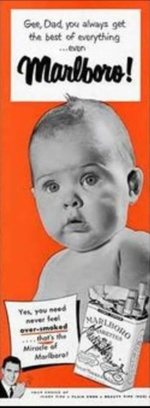
\includegraphics{images/Smoking_SM.png}
	\end{figure}
	
	\subsubsection{Ideals of Beauty}
	During World War 2, with men fighting in the war, images of hard-working women were the dominant image. After the war ended, the ideal of the feminine woman became popular again culminating in the pin-up women. \\
	Pin-Up Art, which is erotic mass produced depictions of women, started being popular. \\
	Alfred C. Kinsley published the two \textbf{Kinsley Reports} on Human Sexuality. These were, at that time, "shocking" revelations. Among them were statistics like:
	\begin{itemize}
		\item{90\% of males and 50\% of females having engaged in sexual intercourse before marriage}
		\item{50\% of males and 26\% of females having commited adultery}
		\item{37\% of males and 13\% of females having had at least one "overt homosexual experience ot orgasm"}
	\end{itemize}
	There is a strange dichotomy in sexuality in America, where it is both repressed but also used to market things. \\
	\subsubsection{Playboy magazine}
	In 1953 the playboy magazine was founded by Hugh Heffner. He chose the bunny as a 'frisky and playful' image. The first cover girl was \textbf{Marilyn Monroe} who caused a huge scandal by posing nude for a calendar. \\
	She was one of the most popular models of this era, being called "Sex Goddess" and "Bombshell". She had a very distinct combination of sexuality and innocence. \\
	\subsection{The Hays Code}
	Going back to Will Hays a movie censor and politican, this code was introduced in 1930, made mandatory in 1934 and abolished in 1968. It regulated what movie makers were allowed to show on television. Among them were:
	\begin{itemize}
		\item{}
	\end{itemize}
	After being abolished in 1968 it was replaced with the system that is still in place today.
	\subsection{Music And Censorship}
	Rock and Roll was heavily censored when it emerged, mainly due to its implied sexuality. \\
	Elvis Presley, the most important Rock n' Roll singer, was known for sexual innuendos. He was known as "Elvis the Pelvis" for his distinct hip movements. Whenever he was shown on television he would be shown from his chest upwards or with a guitar covering him in order for his hips to not be visible. \\
	Other famous Rock n' Roll artists were: 
	\begin{itemize}
		\item{Little Richard}
		\item{Jerry Lee Lewis, called the 'Bad Boy of Rock n' Roll'}
	\end{itemize}
	\subsection{Juvenile Delinquency}
	During that era there was also high criminality among teenagers, mainly in American cities. It was an expression of teenage rebellion. \textbf{James Dean} was one of the icons of this era, starring in 3 influental movies before his untimely death at 24 years. He was considered a "Hipster", a rebel against social and sexual norms by being openly bisexual, listening to jazz and smoking cannabis. \\
	This followed the \textbf{Beat Generation}, a social and literary movement marked by rebellion against norms, which centered on bohemian art communities. It contempted the rules of mainstream society and searched for "blissful illumination".
	\subsection{Pop Art}
	At this time traditional art was also challenged with pop art becoming popular, which is a stylised comic art style of showing "mundane" imagery, like Andy Warhols popular tomato soup imagery.
	\subsection{Neo-Pop}
	With it came Neo-Pop and \textbf{Jeff Koons} who is best known for his aggressive self-merchandising, making sculptures of him having sex with his then wive, an Italian porn star. \\
	\subsection{Conceptual Art}
	Barbara Kruger, an Americna conceptual artist, criticised the superficiality of consumerist culture. She published a book, inofficially titles "I shop, therefore I am". \\
	\subsection{Protest Music}
	At this time Rap and Hip Hop became popular with bands like \textbf{Run-D.M.C.} and \textbf{Public Enemy} being formed. \\

	\section{American Inventions - 17.12.2021}
	In the 1830s the Electric Telegraph was invented and soon later patented by \textbf{Samuel Morse}. The first long-distance telegraph line between Washington D.C. and Baltimore was financed by the U.S. Congress in 1844. The first message transmitted by it was 'What hath God wrought', showing the importance of religion in that area at the time. The invention of the landline was immensely useful for any kind of information transmission but at first was mainly used for the quick transmission of news for jounralistic purposes.
	At the same time the \textbf{Associated Press} was founded. Nowadays there are 1300 Daily Newspapers in the US. The largest by circulation are:
	\begin{itemize}
		\item[6.]{The Washington Post (Center Left)}
		\item[5.]{Los Angeles Times (Center Left)}
		\item[4.]{New York Post (Right)}
		\item[3.]{The New York Times (Center Left)}
		\item[2.]{The Wall Street Journal (Center/Conservative)}
		\item[1.]{USA Today (Centrist)}
	\end{itemize}
	\subsection{Industrial Revolution in the US}
	The US entered the industrial revolution in the 1820s and ended it in the 1870s. This was much later than in Europe where it had already happened in the 1760s. With the industrial revolution came new technologies and new processes of manufactury. \\
	When it did happen in the 1820s the US developed extremely quickly. This was becasue it was very friendly to businesses. There was very little interference from the US government, which practiced a policy of laizzes-faire. There were also very low taxes, which further harbored economic growth. It also limited the liability of owners of companies, which, in case of bankrupcy, were only liable for their own debts and not the debts of the company. \\
	In 1876 Alexander Graham Bell invented the telephone and founded the \textbf{Bell Telephone Company}, later called American Telephone and Telegraph Company, now called AT\&T. In 1904 there were 3 million phones connected in the US and in 1914 they had the highest telephone density in the world. In 1973 Motorola unveiled the first cellular phone. \\
	At the same time \textbf{Thomas Alva Edison} invented direct current and invented the phonograph, the electric generator as well as the light bulb. He also brought lamp systems to New York, San Francisco and Boston. \\
	He was also involved in the technological advancements of films, although not photography. \\
	This was pioneered in France in 1826 with the 'View from the window at le gras', a picture that took 8 hours to develop. The first successful photographic process was the \textbf{Daguerreotype}, which projected the picture on a silvered copper plate. \\
	Photography saw a large surge in popularity with the Civil War, where they were used in Newspapers as proof of what they were reporting. \textbf{The Battle of Gettysburg} was a picture taken by Matthew Brady, depicting people laying dead on a field. \\
	In th 1870s film was arguably invented by Edweard Muybridge when he constructed a flipbook of a galloping horse. While an influental English photographer, he worked in the US. He focused on aesthetics and art without any commercial interest. He was very fascinated with turning still images into something that looked like real life. He published a famous photo series of motion pictures, one of them being a man walking up stairs or a buffalo galloping. \\
	At this time Edison entered the picture who patented the \textbf{Kinetoscope and Kinetograph}. He founded a Movie production studio called \textbf{Black Maria}. He was the first to start making commercial motion pictures in the US in the mid 1890s along with the Lumiére Brothers in France. \\
	His first movie was of two boxing cats, shot in 1894 in Edisons studio. Early films were seldom longer than 1 minute. Only 10 years later did movies already regularly last 6 minutes. \\
	These early beginnings gave rise to the film industry. The first \textbf{Nickelodeon}, small movie theatres, was opened in Pittsburgh in 1905. In 1907 there were already around 8000 of them. In 1910 they already had 26 million viewers per week. \\
	The first major film company was \textbf{Vitagraph} founded in 1897 with a capital of 1000\$ in Brooklyn, then not part of New York City. \\
	\textbf{David Wark Griffith} was the first major filmmaker, with his controversial movie \textbf{The Birth of a Nation}, based on the novel The Klansman, where the members of the Ku Klux Klan rescue captives. This movie was already 190 minutes long. \\
	At this time \textbf{Florence Turner} became the first major star of US movies. She was also known as the Vitagraph Girl. Another star was \textbf{Theda Bara}, also known as Arab Death, an anagram of her name. She was allegedly the daughter of a French artist and his Arabian mistress. Her most famous movie Cleopatra was extremely popular then but the movie itself is unfortunately no longer available. \\
	\subsection{The Academy Award of Merit}
	The Academy Award is organised and overseen by the Academy of Motion Picture Arts and Scienes, which held the first ceremony at a private dinner banquet in Hollywood in 1929. \textbf{Janet Gaynor} was awarded a trophy in three different categories, which was also the only occasion where this happened. Emil Jannings was the first actor, as opposed to actress, to be awarded an academy award. Charlie Chaplin was also awarded honorary awards for two of his movies. \\
	His movie \textbf{The Jazz Singer} was the first sound film. In the movie the words 'Wait a minute. Wait a minute. You ain't heard nothing yet' were the first to be spoken on television \\
	At that time the Hollywood Studio System was very centralised. The production, distribution and exhibiton were all handled by one studio. The 8 large studios at that time were:
	\begin{enumerate}
		\item{Paramount o nthe 8th of May 1912}
		\item{Universal Pictures on the 30th of April 1912}
		\item{United Artists}
		\item{Warner Brothers}
		\item{Columbia Pictures}
		\item{MGM}
		\item{RKO Pictures}
		\item{20th Century Fox}
	\end{enumerate}
	This \textbf{Hollywood Studio System} was put into question by Anti-Trust Laws in the 1940s due it being a massive monopoly without any competition. Few of the large studios survived these Anti-Trust Laws.
	Today there's the \textbf{Big Three} in motion pictures. Columbia Pictures, founded in January 1924, is today a subsidiary of Sony Pictures. \\
	Universal Studios, founded in April 1912, by Carl Laemmle.
	Warner Brothers, the largest film studio by revenue, founded in 1923.With blockbusters like Star Wars, Superman or The Matrix.
	These studios, while the largest by revenue, are not the largest by output, which are outperformed by Nigeran and Indian movie studios, respectively.
	When films became popular, radio stations also had a surge in popularity. KDKA, in Pittsburgh was the first commercial radio station, established in 1920. By the 1940s there were millions of radios but onl about 4000 televisions. \\
	At this time television had not started out yet. While in 1950 only 10\% of American households owned a TV set, it was already 90\% in 1960. Within just 10 years the number of TV sets increased by 80\% in total. \\
	The oldest television station is W2XB, established in 1928. As always they were not immediately commercialised but at first in an experimental state. General Electric started producing television in Schenectady. They had their first regularly scheduled television service in 1928. \\
	In the 1950s a boom of television popularity happened, with radio losing out in popularity. \\
	The three big networks were, and still exist today: 
	\begin{enumerate}
		\item{National Broadcasting Company (NBC)}
		\item{Columbia Broadcasting System (CBS)}
		\item{American Broadcasting Company (ABC)}
	\end{enumerate}
	But over time new ones were established with FOX being founded in 1986. These networks reached as much as 97\% of American households. \\
	\subsection{Atomic Age}
	The Atomic Age is what followed the detonation of the first atom bomb in 1945. \\
	The Manhattan Project was a secret US project to construct the first nuclear bomb. It was led by Julius Robert Oppenheimer, also called the 'Father of the Atomic Bomb'. \\
	The reason why they were vying for atomic bombs, was because they were concerned that the German Reich would soon construct their own Atomic Bomb. Albert Einstein allegedly sent a letter to the government, urging them that the Third Reich would soon have their first atomic bomb. \\
	But they didn't end up using it on the Germans, instead dropping it on Japan. \textbf{Little Boy} was dropped on Hiroshima, killing 166,000 people and only a few days later dropped \textbf{Fat Man} on Nagasaki, killing 80,000 people. \\
	The dropping of the bombs was ordered by president Harry S. Truman. \\
	\subsubsection{Nuclear Arms Race}
	Following this in 1949 the nuclear arms race started with the USSR and the US both developing atomic bombs. \\
	This was soon followed by the \textbf{Hydrogen Bomb}, which can be called the Nuclear Bomb 2.0, 100 times more powerful than its predecessor and five times as hot as the sun. Despite having been tested it was never used to kill people. Instrumental in its development was Edward Teller, American-Austrian physicist. \\
	At that time \textbf{Duck and Cover} spots were produced, starring Bert the Turtle. These commercials were meant to alert people of doing 'the right thing' when the atomic bomb explodes. At this time there was active fear of the other side using atomic bombs to attack them, spurring the construction of fall-out shelters, buried steel tanks to find shelter. \\
	In the 1960s 200,000 American families has family fallout shelters. There were even do-it-yourself shelters that could be built for as little as 200\$ \\
	The rhetoric of this age was, that atomic energy could be used in five sectors:
	\begin{itemize}
		\item{Warfare, as a deterrent}
		\item{Electricity, of using it in nuclear fission}
		\item{Farming, that you could use atomic energy to have things go faster}
		\item{Healing, Using radiation to heal cancer}
		\item{Research, Atomic Energy labs for children}
	\end{itemize}
	These energy labs, called \textbf{Gilbert U-238 Energy Lab} came with a geiger counter and had children handle nuclear substances. It included 'Nuclear Models and samples of radioactive substances as well as an electroscope'. There was, at that time, no awareness of the danger that comes from nuclear radiation. During atomic tests people watched the detonation of atomic bombs in braod daylight without any protection. \\
	Often army troops were only 6 miles away from the blast of an atom bomb. They did not warn people but even encouraged people to come close, presumably to show off their technology. In Las Vegas they even had the detonation of atom bombs as a tourist attraction. \\
	A popular phrase was 'Keep watching the skies', but it did not refer to atomic bombs, but UFO, unidentified flying objects. There was a veritable ufo craze in the 1950s. There were 650 reports of UFO sightings between 1951 nad 1959, though they were always either false alarms or downright manufactured.
	\subsection{Science Fiction}
	At this time Science-Fiction also became popular. The background of this was the arms race between the USA and the USSR. This was caused by events like the \textbf{Sputnik Crisis} as well as the first earth-borne creature, with the dog Leika. \\
	At the same time the first 3-D movie was also released, titled \textbf{The Power of Love} in 1922 though it was not feature length. \\
	The first feature length movie was Bwana Devil released in 1952.
	At this time film also became a spectacular event, being exciting and unknown. This was also prompted by the aims to explore outer space, spurred by John F. Kennedys speech about the \textbf{New Frontier}. The first season of \textbf{Star Trek} took its inspiration from this. NASA had already been established in 1958 by his predecessor to aid in the recrutiment of astronauts. \\
	In 1953 DNA was deciphered by \textbf{James Watson and Francis Crick} and gave rise to genetic engineering and, among other things, the cloned sheep Dolly. \\
	At this time the first large scale digital computer was built called \textbf{ENIAC} developed at the University of Pennsylvania between 1946 and 1955. \\
	The first laptop was unveiled in 1975 by IBM and wieghed 55 pounds, or about 25 kg. \\
	In Silicon Valley, many of the companies instrumental in the establishment of computers like Microsoft and Apple were formed. \\
	In 1989 the World Wide Web was established. In 1993 1\% of digitally transmitted information was internet data. In 2000 it as already 51\% and in 2007 it was 97\%. This also gave rise to the Dot-com bubble, which burst in 2000 and lost many people millions of dollars. \\
	The first smartphone was unveiled in 1994 by IBM and cost 899\$. Apple developed the first modern smartphone in 2007. \\
	With smartphones came selfies, a term first used in 2005. But the first selfie was already taken in 1839 by Robert Cornelius. One  famous selfie was taken with Barrack Obama, David Cameron and Helle-Thorsten Schmid at Nelson Mandela's funeral. There are also animal selfies. In 2011 a monkey took a selfie with David Slaters camera and unwittingly took a selfie. He was later sued by PETA which later settled with him under the condition that he donated 25\% of the revenue made fomr it to animal rights. \\
	
	\section{Civil Rights Movement - 14.01.2022}
	With the end of the American Civil War, slavery too was abolished and the 13th Amendment said that 'Neither slavery nor involuntary servitude [...] shall exist within the United States [...]'. \\
	Following it came the \textbf{Reconstruction Era} from 1865 into the 1880s. Even though slavery was abolished, racism against black people was still widespread.  \\
	\begin{figure}[H]
	\centering
	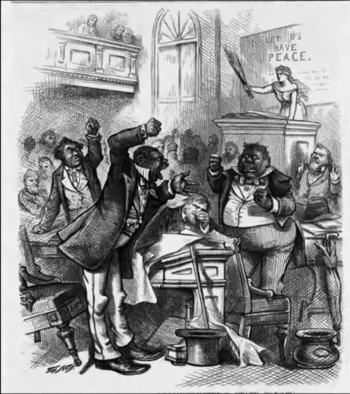
\includegraphics{images/Black_Quarrels.png}
	\end{figure}
	Out of this sentiment came the \textbf{Ku Klux Klan (KKK)} a secretive militant, right-wing organisation intent on 'purifying the American society' through lynchings and pickets. In the 1920s the Klan had an estimated 4.5 million members. By comparison they have between 5000 and 8000 members today. Movies like 'The Birth of a Nation' were very positive towards the Klan and the things it stood for; it was even endorsed by a President. \\
	One of the most well known, but not invented by them, was the slogan \textbf{America First}, which is often still used today for nationalistic purposes. The term itself originates from Woodrow Wilsons presidential campaign of 1916 which at that time had a policy of nationalism and non-interventionism. He argued that they should focus only on themselves and their own well-being. \\
	The slogan was used once again for Donald Trumps presidential race and following his victory also became the slogan of his presidency.
	\subsection{The Progressive Era}
	The Progressive Era, spanning from the 1890s to the 1920s, saw large social reforms. The three main goals were:
	\begin{itemize}
		\item{Environmentalism - The Preservation of Natural Resources}
		\item{Social Welfare - The Improvement of Working Conditions, among other things}
		\item{Civil Rights Activism - Women's and Equal Rights Movements}
	\end{itemize}
	\subsubsection{Environmentalism}
	Yellowstone National Park became the first national park in the world, established in 1872 by the US Congress. It is famous for geysers, like the Old Faithful which erupts approximately every 44 minutes to 2 hours. \\
	Another national park founded during that time is the \textbf{Yosemite National Park}, established in 1890. During this time the preservation of nature and wildlife became a factor. \\
	Another part of the Environmentalism is the \textbf{Green Movement} with the slogan of 'Think Globally, Act Locally' and having annual Earth Days on the 22nd of April. This became a worldwide movement with many Green Parties being formed and also being able to act upon legislation today.
	\subsubsection{Social Welfare}
	At the same time working conditions for workers started to improve dramatically. One such improvement was the effort to end child labour and by 1918 it was abolished in all states of the US. Awareness for the problems of the working class also became more prevalent. Labour unions started regularly organising protest rallies to protest for better rights as workers. One example is the \textbf{Haymarket Riot} of 1886 which resulted in violent outbursts. \\
	Another party formed at that time was the \textbf{Progressive Party}, also called the Bull Moose Party, co-founded by Theodore Roosevelt. It was formed out of the progressive wing of the Republican Party in 1912. In the 1912 presidential elections Roosevelt won 27.4\% of the votes. This was less than Democrat Woodrow Wilson's 42\% but more than Republican William Taft's 23.3\%. This was the first time that a third party scored more than the big 3 parties. \\
	Theodore Roosevelt is also one of the 4 presidents memorialised at Mount Rushmore, sharing it with George Washington, Thomas Jefferson and Abraham Lincoln. \\
	In 1901 the Social Party of America was formed with \textbf{Eugene V. Debs} being its most successful candidate. He ran for presidency five times and at one point received more than 900,000 votes. He was sent to prison in 1919 for speaking out against the war and ran for president from prison, where he again received close to 1 million votes. \\
	One of the nation's heroes of the labour movement since the 1890s was \textbf{Mother Jones}, her real name having been Mary Harris Jones, who emigrated from Ireland at the age of five. She became one of the most prominent union leaders i nthe late 1860s and organised the \textbf{United Mine Workers} union in the 1890s. \\
	As of 2021 more than 40 million people in America are living on food stamps, which is about 12.7\% of the population. This is a figure that has increased dramatically in recent years. Food stamps are part of the Supplemental Nutrition Assistance Program (SNAP) which aids in food purchases for low-income households. \\
	\subsubsection{Civil Rights}
	Starting in the 19th century the women's rights movement gained tractions, demanding equal pay, equal education and full voting rights. In 1848 the \textbf{Seneca Falls Convention} took place and is generally considered the birthplace of the American Women's Movement. The Revolution was a feminist newspaper edited by \textbf{Elizabeth Cady Stanton} and \textbf{Susan B. Anthony}. \textbf{Susan B. Anthony} was the first woman to vote in a presidential election in 1872. This was also the same time when the first woman ran for US President with \textbf{Victoria Woodhull} who was imprisoned for that. She ran on the ticket of the \textbf{Equal Rights Party} together with Frederick Douglass, the most photographed person of that time. Her candidacy was declared illegal and she was sent to prison on election day. Victoria Woodhull was also the first woman to run a brokerage on Wall Street and also the first female editor of a newspaper. She was also an advocate of 'Free Love', which made her very unpopular. \\
	In 1920 the 19th Amendment granted all women the right to vote. At that time 16 states had already allowed women to vote in national elections. This was mainly states in the west as they were trying to get women to move to their states. \\
	In the 1960s \textbf{Betty Friedan} wrote \textit{The Feminine Mystique} which is a sociological study from 1963. She called marriage a 'concentration camp' as you were deprived of many rights of autonomy while in a marriage. \\
	Going back to the Progressive Era, African American Activism became more popular. This had already started with the Abolitionist Movement of the 18th Century with people like Frederick Douglass petitioning for it. \\
	The most famous activist during the 19th century was \textbf{W.E.B du Bois} a historian with Dutch, English and African Ancestors. One of his major works is 'The Souls of Black Folk' published in 1903. He also started the Pan-African Movement when he moved to Kenya. \\
	In the early to mid 20th century African American life was dominated by racial violence and anti-black laws with lynchings being commonplace and \textbf{Jim Crow laws} segregating the races. \\
	These laws saw a complete separation of life between racial groups, providing separate bathrooms, seating space in public transportation and schools, among others. The key phrase of these laws was \textbf{Separate but Equal}, coined by a lawsuit from 1896 titled \textbf{Plessy vs. Ferguson}. In that lawsuit Homer Plessy, officially 1/8 black sued the state as he was considered black by legislation and was denied entry into a whites Louisiana railroad wagon. He lost the lawsuit, which had major ramifications for separation laws as it led to the segregation seen from the Jim Crow Laws. \\
	In the 1950s America was a deeply divided country with both sides protesting against the other. A famous case of lynchings is the killing of Emmet Till, who said 'Bye, baby' to a female shopkeeper. When she told her husband he mutilated and killed him with his friends. 10,000 people attended his open-casket funeral as his mother insisted on people seeing his dead body. They were later declared not-guilty. \\
	In 1964 the KKK killed three civil-rights activists in Mississippi. \textbf{James Earl Chaney, Andrew Goodman and Michael Schwerner} went to Mississippi to protest for civil rights. Following these murders the \textbf{Civil Rights Act} was enacted which outlawed discrimination against women and blacks in the workpalce and public places. In addition the \textbf{Voting Rights Act} was passed which outlawed discriminatory voting practices used against african americans. \\
	Law suits have historically shaped politics in the United States. The lawsuit \textbf{Brown vs. Board of Education} made segregation at public schools illegal. In the lawsuit Oliver Brown's daughter had to walk six blocks to a bus stop to then drive 1 mile to a black segregated school while a white-only school was just seven blocks away. They won and segregation of schools was officially abolished. \\
	Following this landmark lawsuit the \textbf{Little Rock Nine} were the first African American students who attended Little Rock Central High School in 1957. Following threats of lynching, the army was stationed to ensure their safety. \\
	Following Rosa Parks' conviction for not wanting to give up her seat to a white person, the NAACP, the National Association for the Advancement of Coloured People, for a lawsuit. They did not sue but boycotted the bus company for 360 days causing the company such a loss that they stopped the segregation. A key person in this boycott was \textbf{Martin Luther King} who stepped into the limelight, started his policy of civil disobedience, influenced by Mahatma Gandhi. He later gave the famous 'I have a Dream' speech in Washington D.C. \\
	Another prominent figure in African Activism was \textbf{Malcolm X} a more militant supporter of the cause. He helped founding the 'Black Panthers', to combat police brutality. A key smybol of the Black Power Movement was the raised fist whic hfirst happened at the Olympic Games in 1968. \\
	When Trayvon Martin was shot in 2012 by George Zimmerman and subsequently acquitted the Black Lives Matter formed and led to violent protests. Other recent examples of police brutality was the killing of Michael Brown in Ferguson and the death of George Floyd. \\
	Another protest for the same cuase is the \textbf{National Anthem Protest} where people kneel instead of standing while the US Anthem plays for American Football games. It was started by Colin Kaepernick who was later effectively barred from playing in League games. \\
	Presidents during these times were \textbf{Lyndon B. Johnson} who enacted the Civil Rights Act, \textbf{Richard M. Nixon} who was part of the Watergate Scandal and the only president ever to resign from office. Following him was \textbf{Gerald Ford}, nixons Vice-President who automatically took over and immediately pardoned Nixon. And finally \textbf{Jimmy Carter} who at that time was one of the first people to oppose the death penalty. \\
	Other civil rights movements were the \textbf{League of United Latin American Citizens (LULAC)} founded in 1929 and the \textbf{American Indiands Movement (AIM)} founded in 1968. As of 2020 there are 574 different Native American tribes recognised within the US. Another civil rights movement is the \textbf{Mattachine Society} advocating for gay rights founded in 1950 as well as the \textbf{Daughters of Bilits} a lesbian movement. \\
	A notable event in the gay activism movement was the \textbf{Stonewall Riot} from 1969 after a police raid on the Stonewall Inn. This led to the\textbf{Gay Liberation Front} being formed. In the same year another protest movement emerged, called the \textbf{Hippie Movement} that arose as a protest culture and was part of the \textbf{Flower Power Movement}. Centres of the Hippie Movement were New York City and San Francisco. The Background of the Flower Power Movement was the Vietnam War and sparekd by the \textbf{Massacre at My Lai}, where mostly old men, women and children were killed.\\
	
\end{document}